\documentclass{CUP-JNL-DTM}%


%%%% Packages
\usepackage{graphicx}
\usepackage{multicol,multirow}
\usepackage{amsmath,amssymb,amsfonts}
\usepackage{mathrsfs}
\usepackage{amsthm}
\usepackage{rotating}
\usepackage{appendix}
\usepackage[numbers]{natbib}
\usepackage{ifpdf}
\usepackage[T1]{fontenc}
\usepackage{newtxtext}
\usepackage{newtxmath}
\usepackage{textcomp}
\usepackage{xcolor}
\usepackage{lipsum}
\usepackage[colorlinks,allcolors=blue]{hyperref}

\newtheorem{theorem}{Theorem}[section]
\newtheorem{lemma}[theorem]{Lemma}
\theoremstyle{definition}
\newtheorem{remark}[theorem]{Remark}
\newtheorem{example}[theorem]{Example}
\numberwithin{equation}{section}


\jname{Environmental Data Science}
\articletype{DATA PAPER}
%\artid{20}
\jyear{YEAR}
%\jvol{4}
%\jissue{1}
%\raggedbottom


\begin{document}

\begin{Frontmatter}

\title[Article Title]{Data-driven Attributing of Climate Events with \\Climate Index Collection based on Model Data (CICMoD)}

\author[1,3]{Marco Landt-Hayen}\orcid{0000-0003-3606-7760}
\author[1]{Willi Rath}\orcid{0000-0003-1951-8494}
\author[1]{Sebastian Wahl}\orcid{0000-0002-1360-5776}
\author[1]{Nils Niebaum}
\author[1,2]{Martin Claus}\orcid{0000-0002-7525-5134}

\authormark{Landt-Hayen \textit{et al}.}

\address[1]{\orgdiv{Ocean Circulation and Climate Dynamics}, \orgname{GEOMAR Helmholtz Centre for Ocean Research}, \orgaddress{\city{Kiel}, \country{Germany}}} 

\address[2]{\orgname{Christian-Albrechts-Universität zu Kiel}, \orgaddress{\city{Kiel},  \country{Germany}}}

\address[3]{Corresponding author. E-mail: mlandt-hayen@geomar.de}

\keywords{Climate Events, Time Series Forecasting, Artificial Neural Networks, Interpretable ML, Data Mining}

\keywords[MSC Codes]{\codes[Primary]{CODE1}; \codes[Secondary]{CODE2, CODE3}}

\abstract{Machine learning (ML) and in particular artificial neural networks (ANNs) push state-of-the-art solutions for many hard problems e.g., image classification, speech recognition or time series forecasting. In the domain of climate science, ANNs have good prospects to identify causally linked modes of climate variability as key to understand the climate system and to improve the predictive skills of forecast systems. The data science community provides standard data sets for many applications. However, there exists no consistent and comprehensive collection of climate indices covering Earth System dynamics. To attribute climate events in a data-driven way with ANNs, we need sufficient training data, which is often limited for real world measurements. With only short time series available, it is difficult to train ML models and in particular ANNs, that generalize well. Here, we use control runs from Earth System Models over 1,000 years and derive a consistent collection of climate indices. As exemplary applications, we use the data set to predict rainfall in the African Sahel region and El Ni\~{n}o Southern Oscillation with various ML models. But these models tend to produce black box results that are difficult to interpret even by ML experts. We argue that this new data set allows to thoroughly explore techniques from the domain of explainable artificial intelligence to have trustworthy models, that are accepted by domain scientists. Our aim is to build a bridge between the data science community and researchers and practitioners from the domain of climate science to jointly tackle climate change with ML.}

\end{Frontmatter}

\section*{Impact Statement}
Machine learning (ML) models learn from data. To compare and improve ML methods and models, data scientists need standard data sets as benchmark. There exist many standard data sets, like a collection of handwritten digits or images. Our contribution is, to add a consistent and comprehensive collection of climate indices as new data set. This collection can be used to train ML models to understand the climate system with its complex short- and long-term variabilities and to predict climate events. Additionally, the aim is to understand how the models learn and how they come to their conclusion, which is referred to as explainable artificial intelligence. Only if we understand the models in great detail, we gain trust in the results.

\section{Introduction \label{sec:Introduction}}

To apply and compare machine learning (ML) methods and models, there exist standard data sets as benchmark. Among these data sets, we find e.g. a collection of handwritten digits provided by the National Institute of Standards and Technology, referred to as MNIST data set \cite{Lecun1998}. Other data sets contain images, like the CIFAR-10 data set from Canadian Institute for Advanced Research, introduced by Krizhevsky \cite{Krizhevsky2009}, or so-called Fisherfaces, as a collection of human faces in different pose \cite{Belhumeur1997}. These data sets are mostly suitable for classification algorithms. Famous data sets for pattern recognition and clustering applications are e.g. the Iris or Wine data sets, provided by UCI Machine Learning Repository \cite{Murphy1994}, containing attributes for various species of the Iris plant and results of a chemical analysis of wines, respectively. Furthermore, the data science community also provides standard time series collections, like the RAE data set that contains energy consumption time series for various household appliances \cite{Makonin2018}. 

Here, we are interested in describing the underlying dynamics of the Earth System. Real world data is limited to observable features that can be measured in a comprehensive way or that can be reconstructed from sparse measurements. Examples are sea surface temperature (SST), sea level pressure (SLP), sea air temperature (SAT) or geopotential height at various pressure levels, e.g. 500 millibar (Z500). Other features have been measured in the past or are continuously measured only for specific regions by permanent stations that are fixed in place or on trajectories of research cruises, like precipitation (PREC) or sea surface salinity (SSS), respectively. These features reflect some of the main dynamics of the Earth system in form of known climate variabilities, patterns and oscillations, like e.g. Atlantic Multidecadal Oscillation (AMO) \cite{Schlesinger1994}, Southern Annular Mode (SAM) \cite{Gong1999} or El Ni\~{n}o Southern Oscillation (ENSO) \cite{Philander1989}. To model the Earth System, two-dimensional fields can be used to derive specific climate indices that capture the main processes. ML models are then trained on a set of one-dimensional time series instead of two-dimensional fields of various features to reduce computational effort.

For instance, ENSO is a complex phenomenon that can be detected as periodic SST fluctuations in the Tropical Pacific. Several indices are defined to compute the current ENSO phase from area-averaged SST anomalies (SSTA) in certain regions. Morrow et al. \cite{Morrow2010} define the Ni\~{n}o 3.4 index from the Ni\~{n}o 3.4 region (5°N–5°S, 120–170°W) which is often used in the context of ENSO. While ENSO is a large scale driver of the climate system, other indices aim to capture regional variability in specific features, like the Sahel precipitation index (SPI) \cite{Badr2014}. This index measures anomalies of summer rainfall in the African Sahel region (10°N-20°N, 20°W-10°E). Real world climate data is e.g. provided by the Joint Institute for the Study of the Atmosphere and Ocean \cite{JISAO} or the National Oceanic and Atmospheric Administration (NOAA) \cite{NOAA}. However, climate indices are limited in their temporal extend, since consistent real world measurements started only in recent history or measurements are subject of specific research projects that run over a certain period in time. 

Our aim is more general. To better understand existing modes of climate variability and to find new relations, we require a consistent and comprehensive collection of climate indices over the longest possible time span, which favors the use of model data over real world data. Earth System Models (ESMs) aim to model processes of the Earth system in specified temporal and spatial resolution. The Flexible Ocean and Climate Infrastructure (FOCI) \cite{Matthes2020} and the Community Earth System Model (CESM) \cite{Hurrell2013} are both coupled, global climate models that provide state-of-the-art computer simulations of the past, present and future states of the Earth system. The quality of model outputs is evaluated on certain control runs. This can e.g. be done by starting an ESM with pre-industrial conditions from the year 1850 and letting the model unfold its dynamics without external forcing over a desired time span. A control run provides several features. Here, we use the output of FOCI and CESM control runs. In particular, we work with SST, SAT, SLP, Z500, SSS and PREC as two-dimensional fields. From this data, we derive a set of climate indices over 1,000 and 999 years, respectively. The obtained collection of climate indices based on model data (CICMoD) serves as reduced description of the Earth system in a consistent and comprehensive way. 

ML models can then be trained on this CICMoD data set and various methods can be compared to set benchmarks. Relations in the climate systems are often characterized as non-linear and non-stationary \cite{Pak2014,Park2018,Zhang2019}. ML models and methods bear good prospects on this kind of problems. Once we find new relationships in the Earth System, these findings need to be confirmed on real world data to separate facts from model artifacts. A better understanding of causally linked modes within our climate system is essential to tackle climate change and attenuate its impacts. The CICMoD project also opens the door to exploit and explore techniques from the domain of interpretable ML to enhance the explainability of ML models to obtain trustworthy results.

The rest of this work is structured as follows. In Section \ref{sec:Model_Data} we describe FOCI and CESM models and give meta data for model outputs that are used to define climate indices. An overview of all indices included in the CICMoD data set and details on how the indices are derived from raw ESM outputs are given in Section \ref{sec:Climate_Index_Collection}. In section \ref{sec:Application_Results} we show two exemplary applications and use climate indices from CICMoD data set to predict Sahel rainfall and ENSO, respectively. A detailed discussion of all results and a conclusion is found in Section \ref{sec:Discussion_Conclusion}.

\section{Model Data \label{sec:Model_Data}}

In this section, we briefly describe FOCI and CESM models and outline the setup of specific control runs. We present metadata of output files obtained from control runs that serve as basis for deriving climate indices.

[Sebastian: Please add short description of FOCI in general and compared to CESM.]

For FOCI we work with a pre-industrial control run under 1850 climate conditions with no additional external forcing. This run starts from an ocean at rest and runs over 1,500 years. Here, we only use the latter 1,000 years and skip the first 500 years used as spin-up phase to allow the model to find its equilibrium.

[Sebastian: Please add details on corresponding CESM control run.]

From both control runs' output we use Z500, SLP, SST, SSS, SAT and PREC. All features except SSS are provided on a two-dimensional atmospheric latitude-longitude grid. Whereas SSS is originally computed on an ocean grid and is re-gridded to the atmospheric grid. 

[Willi: Please add some details on different grids used here and briefly describe, how we re-grid SSS data.]

Dimensions in latitude and longitude are $96 \times 192$ and $96 \times 144$ for FOCI and CESM output fields, respectively. In any case, the temporal resolution is monthly. Filenames of all output fields are stated in Table \ref{tab:filenames}. Note, that SAT refers to the temperature in 2m height for FOCI output, while CESM output provides termperature directly at the surface.

\begin{table}
\caption{Filenames of control runs' output features for FOCI (upper part) and CESM (lower part)} \label{tab:filenames}

\begin{center}
\begin{tabular}{|c|l|}
\hline
\textbf{Feature} & \textbf{Filename} \\
\hline
Z500 & {\small FOCI1.3-SW038\_echam6\_ATM\_mm\_2350-3349\_geopoth\_pl\_monthly\_50000\_midmonth.nc} \\
SLP & {\small FOCI1.3-SW038\_echam6\_BOT\_mm\_2350-3349\_slp\_monthly\_1\_midmonth.nc} \\
SST & {\small FOCI1.3-SW038\_echam6\_BOT\_mm\_2350-3349\_tsw\_monthly\_1\_midmonth.nc} \\
SSS & {\small FOCI1.3-SW038\_1m\_23500101\_33491231\_grid\_T\_atmos\_grid.nc} \\
SAT & {\small FOCI1.3-SW038\_echam6\_BOT\_mm\_2350-3349\_temp2\_monthly\_1.nc} \\
PREC & {\small FOCI1.3-SW038\_echam6\_BOT\_mm\_2350-3349\_precip\_monthly\_1\_midmonth.nc} \\
\hline
Z500 & {\small B1850WCN\_f19g16\_1000y\_v3.2\_mod-S15-G16.cam2.h0.0001-0999.Z500.midmonth.nc} \\
SLP & {\small B1850WCN\_f19g16\_1000y\_v3.2\_mod-S15-G16.cam2.h0.0001-0999.PSL.midmonth.nc} \\
SST & {\small B1850WCN\_f19g16\_1000y\_v3.2\_mod-S15-G16.cam2.h0.0001-0999.SST.midmonth.nc} \\
SSS & {\small B1850WCN\_f19g16\_1000y\_v3.2\_mod-S15-G16.pop.h.0001-0999.SSS.atmos\_grid.nc} \\
SAT & {\small B1850WCN\_f19g16\_1000y\_v3.2\_mod-S15-G16.cam2.h0.0001-0999.TS.nc} \\
PREC & {\small B1850WCN\_f19g16\_1000y\_v3.2\_mod-S15-G16.cam2.h0.0001-0999.PRECT.nc} \\
\hline

\end{tabular}
\end{center}
\end{table}

\begin{table}
\caption{All indices included in CICMoD data set with their acronyms and spatial domains, ordered by the underlying features} \label{tab:CICMoD}

\begin{center}
\begin{tabular}{|c|l|c|cc|}
\hline
 & & & \multicolumn{2}{c|}{\textbf{Spatial Domain}}\\
 & \textbf{Index} & \textbf{Acronym} & \textbf{Lat in °N} & \textbf{Lon in °E} \\
\hline
Z500 & Southern Annular Mode (PC-based) & SAM\_PC & -90 to -20 & \\
\hline
\multirow{5}{*}{SLP} & Southern Annular Mode (zonal mean) & SAM\_ZM & -65 to -40 & \\
 & Southern Oscillation & SOI & Tahiti & Darwin\\
 & North Atlantic Oscillation (station) & NAO\_ST & Reykjavik & Ponta Delgada\\
 & North Atlantic Oscillation (PC-based) & NAO\_PC & 20 to 80 & -90 to 40\\
 & North Pacific Pattern & NP & 30 to 65 & -160 to 220\\
\hline
\multirow{12}{*}{SST} & Atlantic Multidecadal Oscillation & AMO & 0 to 70 & Atlantic basin\\
 & Pacific Decadal Oscillation & PDO\_PC & 20 to 60 & 120 to 260\\
 & El Ni\~{n}o Southern Oscillation (1+2) & ENSO\_12 & -10 to 0 & 270 to 280\\
 & El Ni\~{n}o Southern Oscillation (3) & ENSO\_3 & -5 to 5 & 210 to 270\\
 & El Ni\~{n}o Southern Oscillation (3.4) & ENSO\_34 & -5 to 5 & 190 to 240\\
 & El Ni\~{n}o Southern Oscillation (4) & ENSO\_4 & -5 to 5 & 160 to 210\\
 & Tropical North Atlantic SSTA & SST\_TNA & -5 to 5 & 160 to 210\\
 & Tropical South Atlantic SSTA & SST\_TSA & -5 to 5 & 160 to 210\\
 & Eastern Subtrop. Indian Ocean SSTA & SST\_ESIO & -5 to 5 & 160 to 210\\
 & Western Subtrop. Indian Ocean SSTA & SST\_WSIO & -5 to 5 & 160 to 210\\
 & Mediterranean Sea SSTA & SST\_MED & -5 to 5 & 160 to 210\\
 & Hurricane main dev. region SSTA & SST\_HMDR & -5 to 5 & 160 to 210\\
\hline
\multirow{4}{*}{SSS} & North Atlantic SSSA & SSS\_NA & 25 to 50 & -50 to -15\\
 & Western North Atlantic SSSA & SSS\_WNA & 25 to 38 & -50 to -40\\
 & Eastern North Atlantic SSSA & SSS\_ENA & 25 to 50 & -40 to -15\\
 & South Atlantic SSSA & SSS\_SA & -22.5 to -10 & -42 to -10\\
\hline
\multirow{6}{*}{SAT} & Northern Hemisphere SATA & SAT\_N\_ALL & 0 to 90 & \\
 & Northern Hemisphere SATA (Ocean) & SAT\_N\_OCEAN & 0 to 90 & Ocean \\
 & Northern Hemisphere SATA (land) & SAT\_N\_LAND & 0 to 90 & land \\
 & Southern Hemisphere SATA & SAT\_S\_ALL & -90 to 0 & \\
 & Southern Hemisphere SATA (Ocean) & SAT\_S\_OCEAN & -90 to 0 & Ocean\\
 & Southern Hemisphere SATA (land) & SAT\_S\_LAND & -90 to 0 & land\\
 \hline
\multirow{1}{*}{PREC} & Sahel Precipitation & PREC\_SAHEL & 10 to 20 & -20 to 10 \\
\hline
\end{tabular}
\end{center}
\end{table}

\section{Climate Index Collection \label{sec:Climate_Index_Collection}}

In this section we gibe an overview of all indices included in the CICMoD data set and reveal details on how the indices are derived. In total, our CICMoD data set consists of 29 climate indices. The indices can be grouped by the underlying model feature. Each feature is discussed separately in the following subsections. We conclude this section with remarks on statistics and pairwise correlation of all indices.

\subsection{Geopotential Height \label{subsec:Z500}}

Geopotential height is a vertical coordinate with reference to Earth's mean sea level. Its contours are used to calculate the geostrophic wind which is of interest for climate dynamics. Here, we choose geopotential height at constant pressure of 500 millibar, referred to as Z500. According to NOAA, Z500 relates to winds in the range between 5,000 and 6,000 meters above mean sea level. We use Z500 to compute the SAM index which relates to the principal mode of variability in the Southern Hemisphere (SH) extratropics. Following the National Center for Atmospheric Research (NCAR) \cite{NCAR}, the SAM index can be obtained as Principle Component (PC) time series of the leading Empirical Orthogonal Function (EOF) of monthly geopotential height anomalies over parts of the SH. SAM has large impact on climate dynamics of the SH, including Australian rainfall and Antarctic surface temperatures \cite{Marshall2007}.  

\subsection{Sea Level Pressure \label{subsec:SLP}}

SLP refers to the air pressure at sea level. Pressure gradients result in winds. Several indices are derived from SLP and its anomalies. In addition to the PC-based version described in Section \ref{subsec:Z500}, the SAM index was originally defined by Gong and Wang \cite{Gong1999} as difference of normalized monthly zonal mean SLP at 40°S and 65°S, respectively. Both versions are included in our CICMoD data set.

The Southern Oscillation Index (SOI) is defined as normalized SLP differences between Tahiti (17°41'S, 149°27'W) and Darwin, Australia (12°27'S, 130°50'E) \cite{Walker1932}. It is used as measure of the large-scale fluctuations in the air pressure between the Western and Eastern Tropical Pacific and is closely related to ENSO. Similarily to SOI, the North Atlantic Oscillation (NAO) index can be computed from SLP as normalized difference between Reykjavik (64°9'N, 21°56'W) and Ponta Delgada (37°45'N, 25°40'W) \cite{Hurrell1995}. Additionally, the NAO index can be obtained as PC time series of the leading EOF of monthly SLP anomalies over the Atlantic sector (20°-80°N, 90°W-40°E) \cite{NCAR}. NAO indices are used to track the seasonal movements of the Icelandic low and Azores high on the Northern Hemisphere (NH). The North Pacific (NP) index measures interannual to decadal variations in the atmospheric circulation. It is derived from area-weighted SLP anomalies in a box bordered by 30°N to 65°N and 160°E to 140°W \cite{Trenberth1994}. Usually, the index focuses on anomalies during November and March. Here we keep full information and provide monthly anomalies for all months of a year.

\subsection{Sea Surface Temperature}

SST is the Ocean temperature close to the surface. SSTA impact the energy transfer at the interface between Ocean and Atmosphere and are of high interest for describing processes in the climate system. Several oscillations are known to exist on individual time scales in the range of years, decades or even longer. AMO refers to a natural variability occurring in the SST of the North Atlantic with a multidecadal period of 60-80 years. AMO is computed from area-weighted SSTA of the North Atlantic \cite{Trenberth2006}. 

The Pacific Decadal Oscillation (PDO) index is obtained as PC time series of the leading EOF of monthly SSTA in the North Pacific basin (20°-60°N, 120°-260°E). PDO resembles ENSO in its spatial pattern. However, ENSO is referred to as an interannual phenomenon while PDO is decadal in scale \cite{Trenberth2013}. 

ENSO is characterized by periodic fluctuations in SSTA in the Tropical Pacific. Its positive and negative phases relate to unusual warm (El Ni\~{n}o) or cold (La Ni\~{n}a) SST, respectively. Tropical Pacific is divided into specific regions, so-calles Ni\~{n}o regions. ENSO indices are then derived from SSTA in the corresponding region. Here, we include Ni\~{n}o 1+2 region as the smallest and eastern-most Ni\~{n}o region where the phenomenon war first recognized by the the local coastal populations. Additionally, we present ENSO indices on Ni\~{n}o 3, 3.4 and 4 regions, respectively. ENSO is a large scale driver of the climate system \cite{Philander1989}. Usually, ENSO indices are smoothed by taking the rolling mean over several months to erase noise. Here, we omit the rolling mean and provide pure SSTA indices instead, to preserve full information. Other regions of interest in the context of climate dynamics related to SSTA are Tropical North Atlantic, Tropical South Atlantic, Eastern Subtropical Indian Ocean, Western Subtropical Indian Ocean, Mediterranean Sea and hurricane main development region, respectively. Corresponding indices are included in our CICMoD data set.

\subsection{Sea Surface Salinity}

SSS measures the amount of salt dissolved in the Ocean surface water and plays an important role in the Ocean cicrulation processes. Furthermore, rainfall on land is largely supplied by evaporation from the Ocean surface water and that evaporation leaves an imprint in SSS. Here, we include several indices derived from SSS anomalies (SSSA) in specific regions of the Atlantic Ocean introduced by Li et al. \cite{Li2016}.

\begin{figure}[!b]
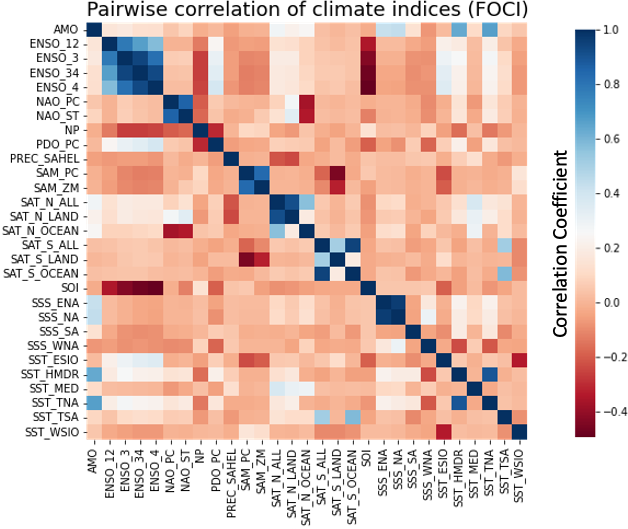
\includegraphics[width=\textwidth]{fig_CICMoD_correlation.png}
\caption{Pairwise correlation coefficients of all CICMoD indices derived from FOCI data.}
\label{fig:CICMoD_correlation}
\end{figure}

\subsection{Sea Air Temperature}

SAT relates to the ability of evaporation, since warmer air has a higher storage capacity for water vapor. Like this, SAT anomalies (SATA) influence the energy transfer at the interface between Ocean and Atmosphere. Here, we track area-averaged monthly SATA on large scales with indices covering complete NH and SH. Additionally, we split NH and SH into land only and Ocean only regions, respectively, and include corresponding indices in our CICMoD data set.

\subsection{Precipitation}

Precipitation has a high impact on society in form of extreme events like flooding caused by heavy rainfall or droughts due to missing or lower as normal rainfall. Exemplary, we include the SPI as measure for rainfall in the African Sahel region. The rainy season in this area is centered on June through October \cite{JISAO}. In its original form, SPI gives a measure for year to year variability of Sahel rainfall as mean over the rainy season. Opposed to that, we provide the SPI as monthly anomalies of rainfall in the Sahel zone (10 to 20°N and 20°W to 10°E) \cite{Badr2014} to preserve full information.

\subsection{CICMoD Data Set}

Table \ref{tab:CICMoD} gives an overview of all 29 indices included in CICMoD data set ordered by the underlying feature. By definition, all indices have zero mean over time, whereas only NAO\_PC, PDO\_PC, SAM\_PC, SAM\_ZM and SOI are normalized to have unit variance by design. If required, normalization of the remaining indices can be done in pre-processing. Exemplary, pairwise correlation coefficients for all indices included in CICMoD data set derived from FOCI model data are shown in Figure \ref{fig:CICMoD_correlation}. Indices derived from CESM data show identical characteristics. ENSO indices are found to be highly correlated, as expected, since these indices are all computed from SSTA in some narrow region of the Tropical Pacific. Additionally, we find station- and PC-based NAO indices to be highly correlated, as well as PC-based SAM and SAM from zonal mean, as these indices describe similar processes. Indices regarding SATA in the NH and SH, respectively, and indices regarding SSS anomalies in the North Atlantic also reveal similarities in terms of high correlation, since by design spatially related features are involved in the computation. Besides that, SOI is found to be negatively correlated to all ENSO indices. 

\section{Application and Results \label{sec:Application_Results}}

In this section we show two exemplary applications of our CICMoD data set to predict Sahel rainfall and ENSO, respectively.

\subsection{Sahel Rainfall \label{subsec:SahelRainfall}}

\begin{figure}[!b]
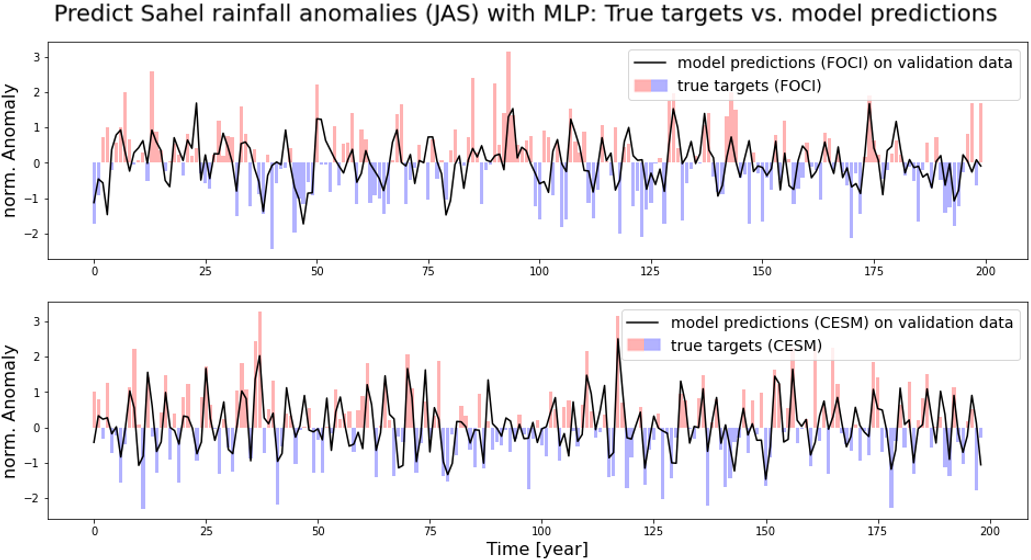
\includegraphics[width=\textwidth]{fig_Sahel_Rainfall_MLP.png}
\caption{Fidelity check on validation data: Sahel rainfall predictions (black line) from MLP models on FOCI data (upper part) and CESM data (lower part), respectively, compared to true targets shown as bar plot}
\label{fig:Sahel_MLP}
\end{figure}

Sahel summer precipitation is observed to be highly variable with floods and droughts occurring on a regular basis. This has a high impact on personal living conditions in that region. Predicting Sahel rainfall and understanding the underlying processes is essential, since it allows taking measures in advance to avoid damage and prevent people from starving. As first application, we use ML models on our CICMoD data set to predict rainfall in the Sahel region. In particular, we apply a linear regression model as baseline and train a multilayer perceptron (MLP). Following the approach of Badr et al. \cite{Badr2014}, we use April to June mean index values as predictors to infer July to September seasonal sum of SPI as target. For FOCI and CESM data, the first 800 years are used as training data, while the remaining 200 and 199 years, respectively, are used for validation. Figure \ref{fig:Sahel_MLP} shows results from MLP models. Results from linear regression are similar and therefore not shown, here. To evaluate model performance, we look at mean squared error (mse) of predictions compared to true targets used as objective or loss function. Additionally, correlation of predicted values and true targets is computed as metric. Corresponding mse and correlation for linear regression and MLP models on FOCI and CESM data, respectively, are shown in Table \ref{tab:Sahel_Eval}.

\begin{table}
\caption{Evaluating model performance for predicting Sahel rainfall with linear regression and MLP models trained on FOCI and CESM data, respectively. Show mse and correlation of predicted values and true targets, separately, for training and validation data} \label{tab:Sahel_Eval}

\begin{center}
\begin{tabular}{|l|c|c|c|c|}
\hline
& \multicolumn{2}{c|}{\textbf{FOCI}} & \multicolumn{2}{c|}{\textbf{CESM}} \\
& \textbf{lin. reg.} & \textbf{MLP} & \textbf{lin. reg.} & \textbf{MLP} \\
\hline
$mse_{train}$ & 0.86 & 0.88 & 0.49 & 0.51 \\
$mse_{val}$ & 0.83 & 0.78 & 0.62 & 0.60 \\
\hline
$correl_{train}$ & 0.55 & 0.53 & 0.70 & 0.69 \\
$correl_{val}$ & 0.50 & 0.52 & 0.68 & 0.69 \\
\hline
\end{tabular}
\end{center}
\end{table}

\subsection{El Ni\~{n}o Southern Oscillation \label{subsec:ENSO}}

\begin{figure}[!b]
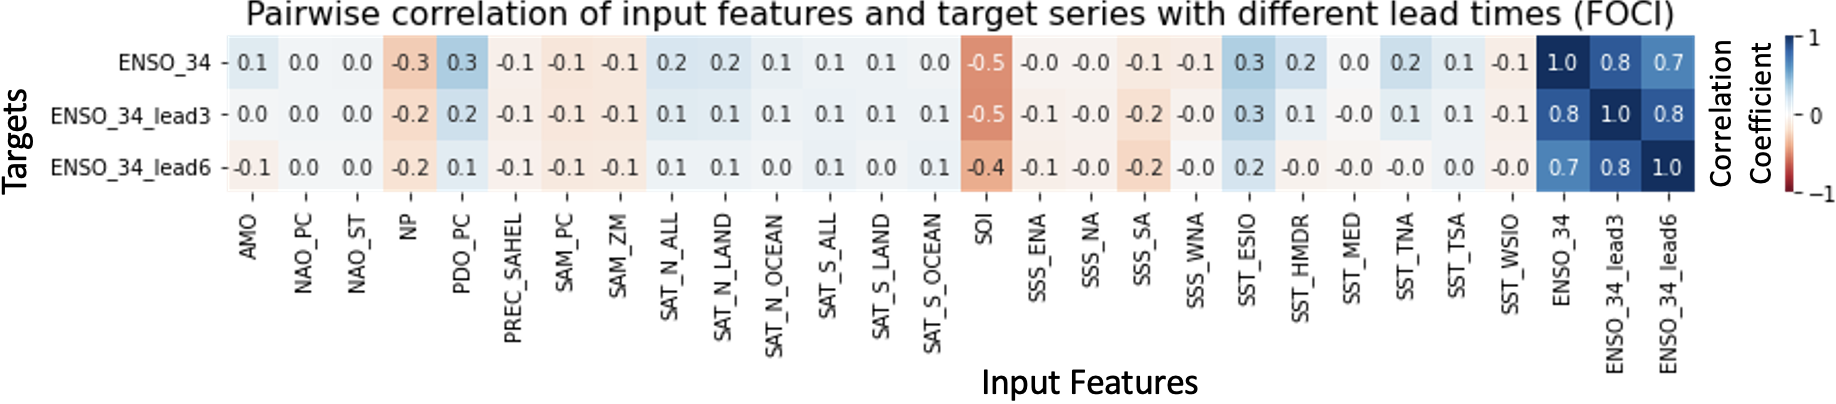
\includegraphics[width=\textwidth]{fig_ENSO_correlation.png}
\caption{Pairwise correlation coefficients of Nino 3.4 index with various time lags (current phase, three and six months into the future) used as targets and input features, both derived from FOCI data}
\label{fig:ENSO_correlation}
\end{figure}

ENSO is the predominant variation of winds and SST in the Tropical Pacific. The positive phase (El Ni\~{n}o) is characterized by unusual warm SST and high SLP, whereas the negative phase (La Ni\~{n}a) relates to unusual cold SST and low SLP. Both events last several months and occur with a period of 2-7 years with varying intensity per period. ENSO tremendously affects those countries bordering the Pacific Ocean. Strong El Ni\~{n}os e.g. correspond to warm weather conditions with heavy rainfalls from April through October causing major flooding along the West coast of South America near Ecuador and the Northern part of Peru \cite{Cai2020}. Consequences of La Ni\~{n}a are e.g. heavy rainfalls over Malaysia, the Philippines and Indonesia. Therefore, knowing the ENSO phase several months in advance is of high interest for society since it allows to take measures to avoid damage and protect people. As second example, we use different ANN models on our CICMoD data set to predict ENSO on various target horizons. In particular, we train convolutional neural networks (CNNs) and long short-term memory (LSTM) models to predict current ENSO phase and ENSO phase three and six months into the future, respectively. Here, targets are derived from ENSO\_34 time series included in CICMoD, which reflects Ni\~{n}o 3.4 index. As input features, we use all remaining indices from our CICMoD data set, excluding other Ni\~{n}o indices due to the high correlation to our targets. Input features are split into sequences of 24 months. We thus try to predict current and future ENSO phases from past two years' conditions. Figure \ref{fig:ENSO_correlation} shows pairwise correlation of targets and input features used in this experiment.

\begin{figure}[]
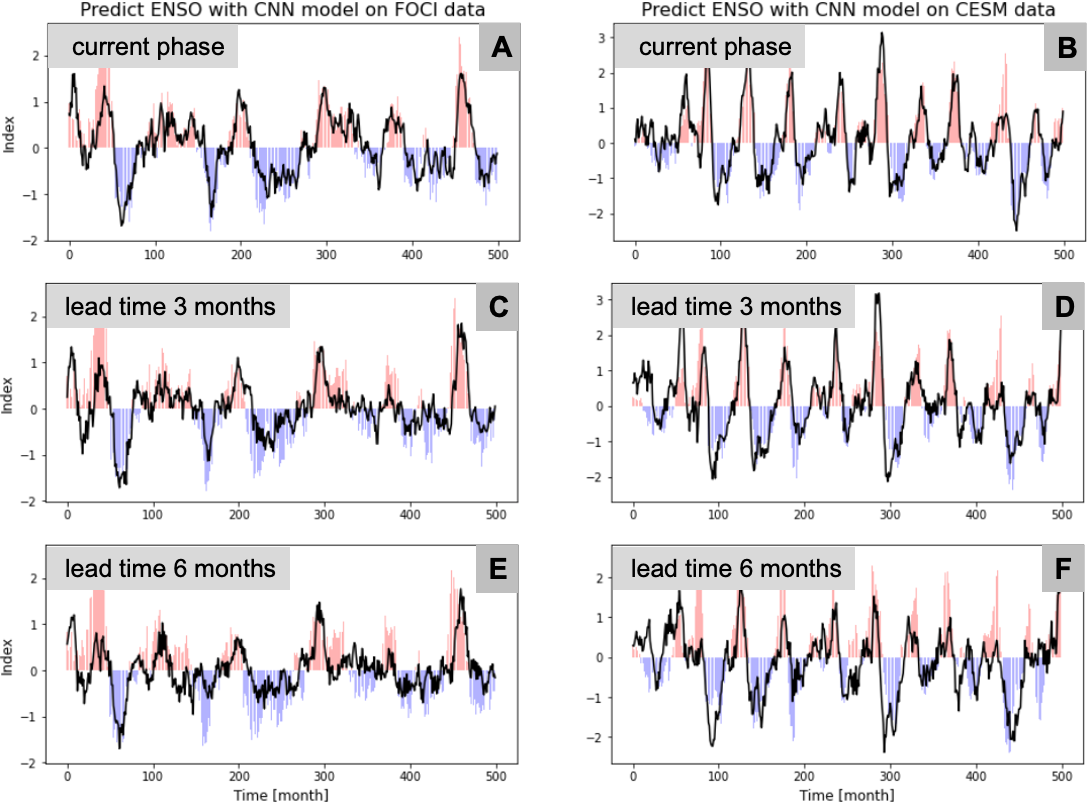
\includegraphics[width=\textwidth]{fig_ENSO_CNN.png}
\caption{Fidelity check on the first 500 months of validation data: Compare predictions (black line) from CNN models on FOCI (left-hand side) and CESM data (right-hand side), respectively, compared to true targets shown as bar plot for various time horizons. A, B: Current phase. C, D: Three months into the future. E, F: Six months into the future}
\label{fig:ENSO_CNN}
\end{figure}

Again, the first 800 years of FOCI and CESM data are used as training data, while the remaining 200 and 199 years, respectively, are used for validation. Figure \ref{fig:ENSO_CNN} shows results from CNN models on the first 500 months of FOCI and CESM validation data, respectively, for various target horizons. To evaluate model performance, we again look at mse and correlation of predictions compared to true targets, as shown in Table \ref{tab:ENSO_Eval}.

\begin{table}
\caption{Evaluating model performance for predicting ENSO with CNN and LSTM models trained on FOCI and CESM data, respectively. Show mse and correlation of predicted values and true targets, separately, for training and validation data. Denote ENSO phase three and six months into the future as lag 3 and lag 6, respectively} \label{tab:ENSO_Eval}

\begin{center}
\begin{tabular}{|ll|c|c|c|c|c|c|}
\hline
 & & \multicolumn{3}{c|}{\textbf{CNN}} & \multicolumn{3}{c|}{\textbf{LSTM}} \\
 & & \textbf{ENSO\_34} & \textbf{lag 3} & \textbf{lag 6} & \textbf{ENSO\_34} & \textbf{lag 3} & \textbf{lag 6} \\
\hline
\multirow{4}{*}{\textbf{FOCI}} & $mse_{train}$ & 0.16 & 0.21 & 0.27 & 0.16 & 0.23 & 0.28 \\
 & $mse_{val}$ & 0.24 & 0.37 & 0.47 & 0.26 & 0.41 & 0.53 \\
 & $correl_{train}$ & 0.84 & 0.79 & 0.72 & 0.84 & 0.77 & 0.71 \\
 & $correl_{val}$ & 0.81 & 0.68 & 0.56 & 0.79 & 0.64 & 0.47 \\
\hline
\multirow{4}{*}{\textbf{CESM}} & $mse_{train}$ & 0.20 & 0.31 & 0.42 & 0.20 & 0.32 & 0.41 \\
 & $mse_{val}$ & 0.29 & 0.48 & 0.65 & 0.30 & 0.50 & 0.73 \\
 & $correl_{train}$ & 0.88 & 0.80 & 0.72 & 0.88 & 0.79 & 0.72 \\
 & $correl_{val}$ & 0.84 & 0.72 & 0.59 & 0.83 & 0.70 & 0.56 \\
\hline
\end{tabular}
\end{center}
\end{table}

\section{Discussion and Conclusion \label{sec:Discussion_Conclusion}}

In this work, we introduce a consistent and comprehensive collection of climate indices. The collection is consistent in a sense that we use the output of ESM control runs to derive all indices. For FOCI and CESM control runs, we have 1,000 and 999 years of monthly data, respectively, as big advantage compared to real world data, since ML models require sufficient training data. And the collection is comprehensive as we include a broad selection of known patterns, oscillations and variabilities of the Earth system. The index collection is not complete since we focus on processes within the Atmosphere, in the upper Ocean and at the interface of Ocean and Atmosphere. However, our CICMoD data set serves as basis. Additionally, we provide an open-source framework that allows to be extended and customized to individual needs including the application to additional ESMs. This opens the door for collaborations in many ways. Our new data set allows researchers from the data science community to adapt existing ML models and develop new ML methods to tackle problems from the domain of climate science and get a deeper understanding of the Earth system. This requires involving scientists and practitioners from the domain of climate science.

In this work, we apply several ML models and use our CICMoD data set to predict Sahel rainfall and ENSO, respectively. In particular, we compare linear regression and to MLP models to predict SPI. Results are shown in Section \ref{subsec:SahelRainfall}. Linear regression models perform slightly better on training data in terms of lower mse combined with higher correlation of predictions and true targets, while MLP models show better performance on validation data, hence generalize better on unseen data. Comparing FOCI and CESM, we find significantly lower mse and higher correlation for linear regression and MLP models trained on indices derived from CESM data. As future work, these differences need to be further investigated. 

As second example, we predict current ENSO phase and ENSO phase three and six months into the future with CNN and LSTM models, respectively. Targets are derived from Ni\~{n}o 3.4 index and as predictors we use all remaining indices, excluding Ni\~{n}o indices. Input features and targets are found to be mostly uncorrelated with correlation coefficients in the the range of -0.5 and 0.4. Results are shown in Section \ref{subsec:ENSO}. We find a higher frequency of ENSO events in time series derived from CESM data, compared to FOCI. Still, periodicity for for El Ni\~{n}o events falls in the expected range of 2-7 years for both models. 

Overall, our CNN models slightly outperform LSTM models for predicting ENSO. Again, we look at mse and correlation for evaluating model performance. The longer the target horizon, the worse the model performance in terms of higher mse and lower correlation, as expected, since ENSO is a complex phenomenon that hinders long-term prediction beyond several months. As for Sahel rainfall prediction, our ML models perform better on indices derived from CESM data, compared to FOCI, which needs to be further investigated in future work.

ESMs aim to model Earth system dynamics. Different ESMs have their individual strengths and weaknesses. For our CICMoD data set, we use two distinct ESMs to derive all indices. This allows to separate facts from model artifacts. Whenever we find some relation in one model context, we may try to reproduce our findings on the other model's data to gain trust before repeating our experiments on real world data. Like this, our CICMoD data set can help to reveal blind spots in ESMs and to find new causally linked modes of the real world climate system. CICMoD as new standard data set opens the door for exploring methods of explainable artificial intelligence (xAI). As further work we plan to combine CICMoD with some xAI toolbox to be used for data science competitions to tackle climate change and push the understanding of the climate system in a playfull way.

\begin{Backmatter}

\paragraph{Funding Statement}
This work was supported by the Helmholtz School for Marine Data Science (MarDATA) funded by the Helmholtz Association (Grant HIDSS-0005).

\paragraph{Competing Interests}
The authors declare none.

\paragraph{Data Availability Statement}
The software project including the current release of our CICMoD data set is hosted on GitHub: \url{https://github.com/MarcoLandtHayen/climate_index_collection}. Furthermore, we reference a Docker container providing a Python environment with Jupyter notebooks, Tensorflow and climate\_index\_collection as pre-installed python package. Exemplary applications of CICMoD data set to predict ENSO and Sahel rainfall are stored in a separate GitHub repository \url{https://github.com/MarcoLandtHayen/cicmod_application}. Raw data is stored on Zenodo: \url{https://doi.org/10.5281/zenodo.7060386}.

\paragraph{Ethical Standards}
The research meets all ethical guidelines, including adherence to the legal requirements of the study country.

\paragraph{Author Contributions}
Conceptualization: M.L.H.; W.R.; M.C. Methodology: M.L.H.; W.R.; N.N. Data curation: M.L.H.; S.W. Data visualisation: M.L.H.; N.N. Writing original draft: M.L.H.; W.R.; S.W. All authors approved the final submitted draft.

\begin{thebibliography}{}
\bibitem{Lecun1998}
\textbf{Lecun Y., Botou L., Bengio Y. and Haffner P.} (1998) Gradient-based learning applied to document recognition, \textit{IEEE} \textit{86}(11), {2278}--{2324}.

\bibitem{Krizhevsky2009}
\textbf{Krizhevsky, A.} (2009) Learning Multiple Layers of Features from Tiny Images \url{https://www.cs.toronto.edu/~kriz/learning-features-2009-TR.pdf}.

\bibitem{Belhumeur1997}
\textbf{Belhumeur P.N., Hespanha J.P. and Kriegman D.J.} (1997) Eigenfaces vs. Fisherfaces: recognition using class specific linear projection, \textit{IEEE Transactions on Pattern Analysis and Machine Intelligence} \textit{19}(7), {711}--{720}.

\bibitem{Murphy1994}
\textbf{Murphy P. and Aha D.} (1994) UCI repository of machine learning databases.

\bibitem{Makonin2018}
\textbf{Makonin S., Wang Z.J. and Tumpach C.} (2018) RAE: The Rainforest Automation Energy Dataset for Smart Grid Meter Data Analysis, \textit{Data} \textit{3}(1):8. 

\bibitem{Schlesinger1994}
\textbf{Schlesinger M.E. and Ramankutty N.} (1994) An oscillation in the global climate system of period 65-70 years, \textit{Nature} \textit{367}, {723}--{726}.

\bibitem{Gong1999}
\textbf{Gong D. and Wang S.} (1999) Definition of Antarctic oscillation index, \textit{Geophysical Research Letters} \textit{26}(4), {459}--{462}.

\bibitem{Philander1989}
\textbf{Philander S.G.} (1989) El Ni\~{n}o, La Ni\~{n}a, and the Southern Oscillation, vol. 46, \textit{Academic Press}, San Diego, USA.

\bibitem{Morrow2010}
\textbf{Morrow R., Ward M.L., Hogg A.McC. and Pasquet S.} (2010) Eddy response to Southern Ocean climate modes, \textit{Journal of Geophysical Research} \textit{115}.

\bibitem{Badr2014}
\textbf{Badr H.S., Zaitchik B.F. and Guikema S.D.} (2014) Application of Statistical Models to the Prediction of Seasonal Rainfall Anomalies over the Sahel, \textit{Journal of Applied Meteorology and Climatology} \textit{53}(3), {614}--{636}.

\bibitem{JISAO} 
\textbf{Joint Institute for the Study of the Atmosphere and Ocean}, \url{http://research.jisao.washington.edu/data/}.

\bibitem{NOAA}
\textbf{National Oceanic and Atmospheric Administration}, \url{https://psl.noaa.gov/data/climateindices/}.

\bibitem{Matthes2020}
\textbf{Matthes K., Biastoch A., Wahl S., Harlaß J., Martin T., Brücher T., Drews A., Ehlert D., Getzlaff K., Krüger F., Rath W., Scheinert M., Schwarzkopf F.U.,  Bayr T., Schmidt H. and Park W.} (2020) The Flexible Ocean and Climate Infrastructure version 1 (FOCI1): mean state and variability, \textit{Geoscientific Model Development} \textit{13}(6), {2533}--{2568}.

\bibitem{Hurrell2013}
\textbf{Hurrell J.W., Holland M.M., Gent P.R., Ghan S., Kay J.E., Kushner P.J., Lamarque J.-F., Large W.G., Lawrence D., Lindsay K., Lipscomb W.H., Long M.C., Mahowald N., Marsh D.R., Neale R.B., Rasch P., Vavrus S., Vertenstein M., Bader D., Collins W.D., Hack J.J., Kiehl J. and Marshall S.} (2013) The Community Earth System Model: A framework for collaborative research, \textit{Bulletin of the American Meteorological Society}, \textit{94}, {1339}--{1360}.

\bibitem{Pak2014} 
\textbf{Pak G., Park Y.-H., Vivier F., Kwon Y.-O. and Chang K.-I.} (2014) Regime-Dependent Nonstationary Relationship between the East Asian Winter Monsoon and North Pacific Oscillation, \textit{Journal of Climate} \textit{27}(21), {8185}--{8204}.

\bibitem{Park2018} 
\textbf{Park Y.-H., Kim B.-M., Pak G., Yamamoto M., Vivier F. and Durand I.} (2018) A key process of the nonstationary relationship between ENSO and the Western Pacific teleconnection pattern,  \textit{Scientific Reports}, \textit{8}(9512).

\bibitem{Zhang2019} 
\textbf{Zhang W., Mei X., Geng X., Turner A.G. and Jin F.-F.} (2019) A Nonstationary ENSO–NAO Relationship Due to AMO Modulation, \textit{Journal of Climate}, \textit{32}(1), {33}--{43}.

\bibitem{NCAR}
\textbf{National Center for Atmospheric Research}, \url{https://ncar.ucar.edu}.

\bibitem{Marshall2007}
\textbf{Marshall G.J.} (2007) Half-century seasonal relationships between the Southern Annular mode and Antarctic temperatures, \textit{International Journal of Climatology}, \textit{27}(3), {373}--{383}.

\bibitem{Walker1932}
\textbf{Walker G.T. and Bliss E.W.} (1932) World Weather V., \textit{Memoirs of the Royal Meteorological Society}, \textit{4}, {53}--{84}.

\bibitem{Hurrell1995}
\textbf{Hurrell J.W.} (1995) Decadal Trends in the North Atlantic Oscillation: Regional Temperatures and Precipitation, \textit{Science}, \textit{269}(5224), {676}--{679}.

\bibitem{Trenberth1994}
\textbf{Trenberth K.E. and Hurrell J.W.} (1994) Decadal atmosphere-ocean variations in the Pacific, \textit{Climate Dynamics}, \textit{9}(6), {303}--{319}.

\bibitem{Trenberth2006}
\textbf{Trenberth K.E. and Shea D.J.} (2006) Atlantic hurricanes and natural variability in 2005, \textit{Geophysical Research Letters}, \textit{33}(12).

\bibitem{Trenberth2013}
\textbf{Trenberth K.E. and Fasullo J.T.} (2013) An apparent hiatus in global warming?, \textit{Earth's Future}, \textit{1}(1), {19}--{32}.

\bibitem{Li2016}
\textbf{Li L., Schmitt R.W., Ummenhofer, C.C. and Karnauskas K.B.} (2016) North Atlantic salinity as a predictor of Sahel rainfall, \textit{Science Advances}, \textit{2}(5).

\bibitem{Cai2020}
\textbf{Cai W., McPhaden M.J., Grimm A.M., Rodrigues R.R., Taschetto A.S., Garreaud R.D., Dewitte B., Poveda G., Ham Y.-G., Santoso A., Ng B., Anderson W., Wang G., Geng T., Jo H.-S., Marengo J.A., Alves L.M., Osman M., Li S., Wu L., Karamperidou C., Takahashi K. and Vera C.} (2020) Climate impacts of the El Ni\~{n}o-Southern Oscillation on South America, \textit{Nature Reviews Earth \& Environment}, \textit{1}, {215}--{231}.

\end{thebibliography}

\end{Backmatter}

\end{document}
